% ============================================================
%  SUPPLEMENTARY FIGURES S18--S22: Hyphae Morphological Analysis
%  For: "Fungal Hyphae as Distributed Hygroscopic Sinks"
% ============================================================


% ── S18: FFT Spectral Analysis + Cross-Validation ──

\begin{figure}[H]
\centering
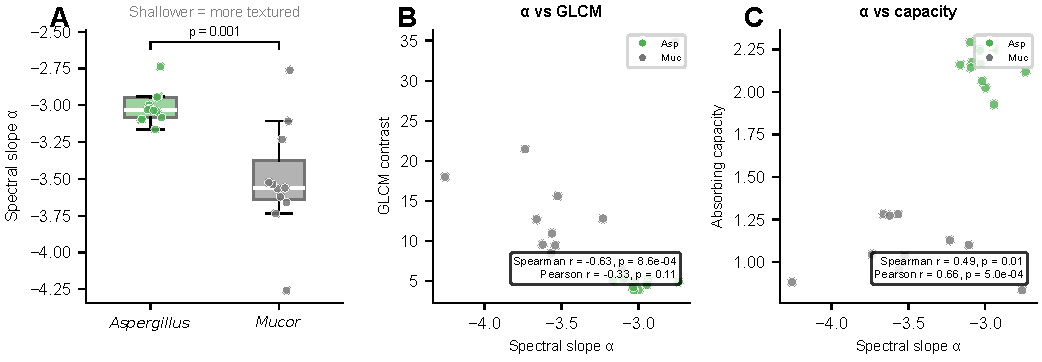
\includegraphics[width=\textwidth]{FigureHyphae/figures/figS18_fft_analysis.pdf}
\caption{\textbf{FFT spectral analysis cross-validates morphological metrics.}
Tile-based 2D FFT ($256 \times 256$~px tiles, 128~px stride, Hanning
window) applied to all macro-scale brightfield colony-surface
photographs (single-plane, not focus-stacked).
\textbf{(A)}~Mean radial power spectra for \textit{Aspergillus}
(green, $n = 13$) and \textit{Mucor} (gray, $n = 11$).
Shaded region: frequency band used for slope fitting
(0.02--0.40~cycles/px).  \textit{Aspergillus} retains more power at
high spatial frequencies, indicating finer-grained surface texture.
\textbf{(B)}~Spectral slope $\alpha$:
\textit{Aspergillus} = $-3.01 \pm 0.11$,
\textit{Mucor} = $-3.51 \pm 0.38$
(Welch's $t$-test, $p = 0.001$, $d = 1.85$;
Mann--Whitney $U = 130$, $p = 0.0008$).
Shallower slope indicates more sub-resolution surface roughness ---
consistent with the bumpy texture of packed conidial chains versus
the smooth surfaces of \textit{Mucor} sporangiophores.
\textbf{(C)}~Cross-validation: $\alpha$ versus GLCM contrast across
all ROIs (Spearman $r = -0.63$, $p = 0.0009$).  Two independent
texture methods (frequency-domain and spatial-domain) converge on the
same genus ordering.  Spearman is reported because the relationship
is monotonic but the Pearson estimate is sensitive to a single
high-contrast \textit{Mucor} ROI; Spearman is robust to that
leverage point.
\textbf{(D)}~$\alpha$ versus absorbing capacity
(Spearman $r = 0.49$, $p = 0.014$).  Colonies with shallower spectral
slope (more textured surfaces) also present higher absorbing capacity,
linking sub-resolution roughness to effective vapor-sink strength.
Spearman is reported here for the same robustness reason as in panel~C.}
\label{fig:supp_fft}
\end{figure}


% ── S19: Light Microscopy Hessian Tubeness ──

\begin{figure}[H]
\centering
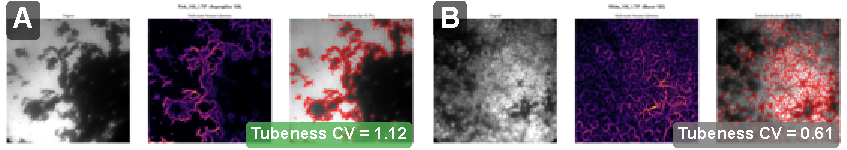
\includegraphics[width=\textwidth]{FigureHyphae/figures/figS19_hessian_lm.pdf}
\caption{\textbf{Multi-scale Hessian tubeness on light microscopy.}
Representative 10$\times$ fields: \textit{Aspergillus}
(Pink\_10X\_1.TIF, \textbf{A}) and \textit{Mucor}
(White\_10X\_1.TIF, \textbf{B}).
Each 4-panel overlay shows: original transmitted-light image (top-left);
multi-scale Hessian tubeness response ($\sigma = 1, 2, 4, 8, 16$~px,
maximum across scales; inferno colormap, top-right); detected tubular
structures (red overlay, bottom-left); internal classification
(blue = solid tissue, yellow = internal pores, bottom-right).
Hessian tubeness selectively responds to elongated filamentous structures.
\textit{Mucor}'s sparse hyphal network produces a uniform, high
tubeness response (foreground fraction = 0.276), while
\textit{Aspergillus}'s dense conidial masses register low tubeness
except at filamentous edges (foreground fraction = 0.185),
consistent with packed rather than filamentous architecture.
The Hessian tubeness ``foreground fraction'' reported here is
intentionally selective for filamentous structures and rejects
\textit{Aspergillus}'s dense conidial cores; this differs from
the adaptive-threshold tissue fraction $f_\mathrm{tissue}$
reported in Supplementary Fig.~\ref{fig:supp_capacity}A
($f_\mathrm{tissue,Asp} = 0.300 > f_\mathrm{tissue,Muc} = 0.258$),
which captures all dark tissue including cores.
\textit{Aspergillus}'s lower Hessian-foreground but higher
adaptive-tissue fraction is internally consistent and is the
underlying reason its tubeness CV is high
(Supplementary Fig.~\ref{fig:supp_tubcv}).
This structural distinction underlies the morphological metrics
in Fig.~\ref{fig:architecture}C--F.}
\label{fig:supp_hessian}
\end{figure}


% ── S20: Erosion Demonstration ──

\begin{figure}[H]
\centering
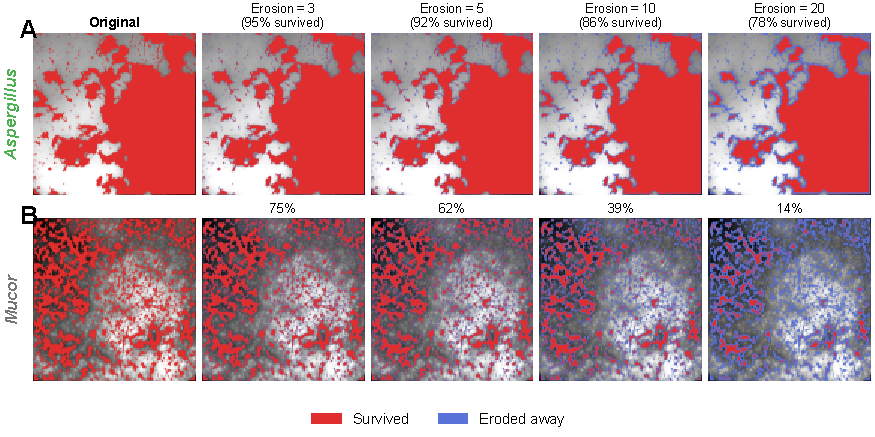
\includegraphics[width=\textwidth]{FigureHyphae/figures/figS20_erosion_demo.pdf}
\caption{\textbf{Progressive morphological erosion.}
Adaptive-segmented tissue masks subjected to 0, 2, 5, 10, and 20
iterations of binary erosion.  Red = tissue surviving erosion;
blue = tissue eroded away.
\textbf{(A)}~\textit{Aspergillus} (Pink 10$\times$).  Dense conidiospore
cores persist through 20 iterations (survival at 10
iterations = 86\%).
\textbf{(B)}~\textit{Mucor} (White 10$\times$).  Thin hyphal filaments
are substantially eroded by 10 iterations
(survival at 10 iterations = 39\%).
Erosion survival (Fig.~\ref{fig:architecture}F) quantifies structural
persistence: thick, packed tissue withstands more erosion cycles than
thin filaments.
Overall: \textit{Aspergillus} = $0.791 \pm 0.103$,
\textit{Mucor} = $0.372 \pm 0.025$
(Welch's $t$-test, $p = 7.9 \times 10^{-5}$, $d = 4.75$;
Mann--Whitney $U = 18$, $p = 0.024$ --- bounded by $n_a = 6$, $n_m = 3$).
Erosion survival values reported in Fig.~\ref{fig:architecture}F
and the genus-level mean above are the per-ROI tissue-retention
fraction at erosion iteration~10, averaged across ROIs
($n = 6$ \textit{Aspergillus}, $n = 3$ \textit{Mucor}).}
\label{fig:supp_erosion}
\end{figure}


% ── S21: Hessian Tubeness CV ──

\begin{figure}[H]
\centering
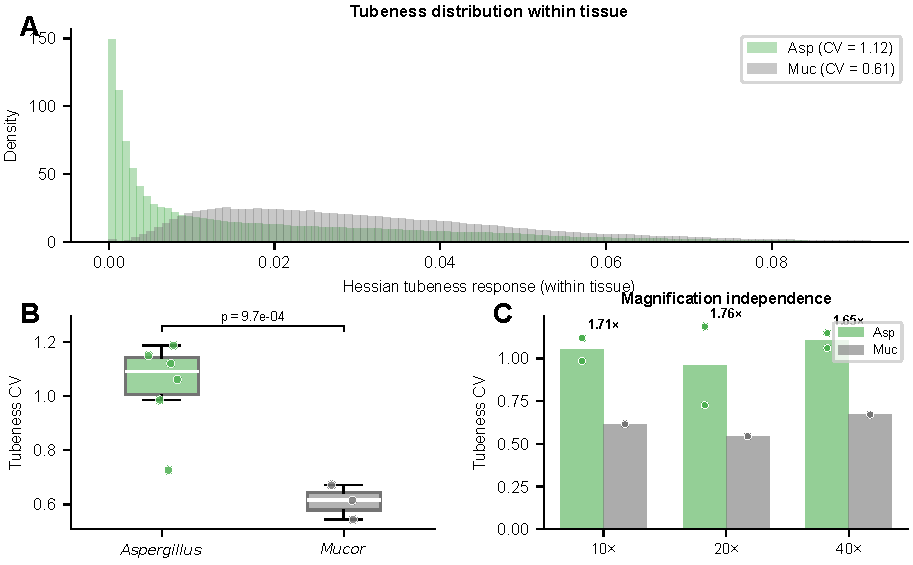
\includegraphics[width=\textwidth]{FigureHyphae/figures/figS21_tubeness_cv.pdf}
\caption{\textbf{Hessian tubeness CV derivation.}
\textbf{(A)}~Distribution of multi-scale Hessian tubeness response
within tissue pixels for one representative ROI per genus
(\textit{Aspergillus}, green, single-ROI CV~=~1.12; \textit{Mucor},
gray, single-ROI CV~=~0.61); the all-image means are reported
in panel~B.
Dashed lines mark means.  \textit{Aspergillus} tissue has a broader,
more heterogeneous distribution---reflecting a mix of solid conidial
cores (low tubeness) and filamentous edges (high tubeness)---while
\textit{Mucor} tissue is narrowly distributed around a single
filamentous mode.  The \textit{Aspergillus} distribution is
strongly bimodal (a zero-inflated peak from solid conidial cores
plus a high-tubeness tail from filamentous edges), so the high CV
reflects this two-mode structure rather than a wider unimodal
distribution.
\textbf{(B)}~Tubeness CV across all light-microscopy images:
\textit{Aspergillus} = $1.04 \pm 0.17$,
\textit{Mucor} = $0.61 \pm 0.06$
(Welch's $t$-test, $p = 9.7 \times 10^{-4}$, $d = 2.93$;
$n = 6$ vs.\ $n = 3$).  Mann--Whitney $U$ is bounded by
$p \geq 0.024$ at $n_a = 6$, $n_m = 3$ (limited by sample size);
Welch's $t$ is reported as primary because the per-image tubeness
CV is approximately Gaussian within group.
The CV is computed within a class-specific adaptive-threshold
tissue mask; replacing the class-specific operator with a single
universal segmentation reduces the Asp/Muc ratio to $1.20$
($p = 0.17$), see Methods for the biological motivation
and Results for the universal-segmentation control.
\textbf{(C)}~Magnification independence: the Asp/Muc ratio is
preserved at $1.71\times$ ($10\times$), $1.76\times$ ($20\times$),
and $1.65\times$ ($40\times$), confirming that the metric reflects
intrinsic morphological character rather than imaging scale.}
\label{fig:supp_tubcv}
\end{figure}


% ── S22: Absorbing Capacity + SSA ──

\begin{figure}[H]
\centering
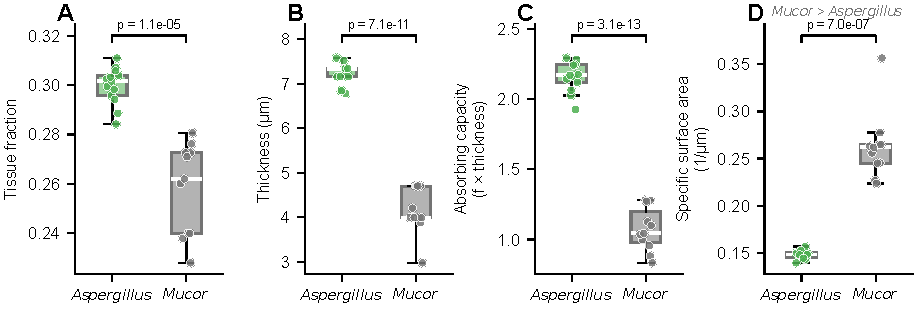
\includegraphics[width=\textwidth]{FigureHyphae/figures/figS22_absorbing_capacity.pdf}
\caption{\textbf{Absorbing capacity decomposition and specific surface area.}
Per-ROI strip charts for the components of absorbing capacity
$\mathcal{A} = f_\mathrm{tissue} \times d_\mathrm{structure}$
(Fig.~\ref{fig:architecture}H).
\textbf{(A)}~Tissue fraction $f_\mathrm{tissue}$:
\textit{Aspergillus} = $0.300 \pm 0.008$,
\textit{Mucor} = $0.258 \pm 0.019$
(ratio = 1.16, $p = 1.1 \times 10^{-5}$).
\textbf{(B)}~Structure thickness $d_\mathrm{structure}$
(median distance transform, \textmu m):
\textit{Aspergillus} = $7.21 \pm 0.26$,
\textit{Mucor} = $4.16 \pm 0.53$
(ratio = 1.73, $p = 7.1 \times 10^{-11}$).
\textbf{(C)}~Absorbing capacity $\mathcal{A}$:
\textit{Aspergillus} = $2.16 \pm 0.11$,
\textit{Mucor} = $1.07 \pm 0.16$
(ratio = 2.01, $d = 8.22$, $p = 3.1 \times 10^{-13}$).
Their product predicts the measured $\delta$ ratio (2.13) within 6\%.
\textbf{(D)}~Specific surface area (tissue--air boundary per tissue area):
\textit{Mucor} = $0.262 \pm 0.035$~\textmu m$^{-1}$,
\textit{Aspergillus} = $0.148 \pm 0.005$~\textmu m$^{-1}$
($p < 10^{-6}$).
Despite $1.78\times$ higher surface-to-volume ratio,
\textit{Mucor} is the weaker sink: total hygroscopic mass per colony
footprint, not surface-to-volume ratio, determines effective sink strength.
$n = 13$~\textit{Aspergillus}, $n = 11$~\textit{Mucor} ROIs.}
\label{fig:supp_capacity}
\end{figure}


% ── S23: Segmentation Threshold Sensitivity ──

\begin{figure}[H]
\centering
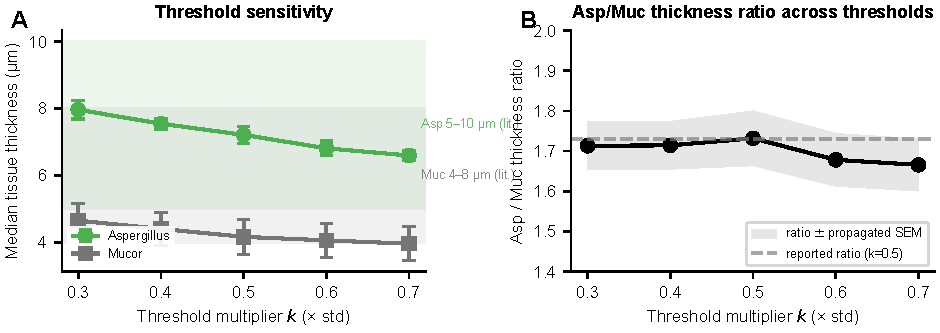
\includegraphics[width=\textwidth]{FigureHyphae/figures/figS_seg3d_sensitivity.pdf}
\caption{\textbf{Segmentation threshold sensitivity for macro-scale colony-surface masks.}
Adaptive dark-response thresholding (smooth $\sigma = 1$~px, local
mean $\sigma = 32$~px) was swept over threshold multipliers
$k = 0.3$ to $0.7\,\times$~std on the same 13~\textit{Aspergillus}
and 11~\textit{Mucor} ROIs used in Fig.~\ref{fig:architecture}.
\textbf{(A)}~Median tissue thickness as a function of $k$ for both
genera (mean $\pm$ std across ROIs).  Shaded bands: published
hyphal-diameter ranges
(\textit{Aspergillus} conidiophore stipe and conidial-chain width
5--10~\textmu m, green; \textit{Mucor} sporangiophore-segment width
4--8~\textmu m, gray).  Both genera fall within their published
ranges across the entire sweep, supporting the calibration choice.
\textbf{(B)}~Asp/Muc thickness ratio is stable at $1.67$--$1.73$
across the full sweep ($k = 0.3$--$0.7$), demonstrating that the
reported $1.73\times$ separation is not an artifact of the chosen
threshold.  The Welch $p$-value remains $< 2.4 \times 10^{-9}$
at every threshold tested.  Tabulated values are in
\texttt{segmentation\_sensitivity.csv} (OSF deposit).}
\label{fig:supp_seg3d}
\end{figure}
